\chapter{Anwendung von NLP in IT-Prozessen}
\label{cha:ApplicationsForNLPinProcesses}
\section{Allgemeines}

In diesem Kapitel wird erläutert, wie \textit{Natural Language Processing} in ausgewählten IT-Prozessen Anwendung finden kann, sowie die Verbesserungen die dadurch erwartet werden. Es wird darauf eingegangen, welche technischen Limitierungen bzw. welche Probleme bei der Anwendung von \textit{NLP} entstehen, sowie eine kurze Bewertung bezüglich der Machbarkeit abgegeben.

Für die Analyse der Anwendungen von \textit{NLP}, wird im ersten Schritt der Ist-Zustand des Prozesses analysiert. Dazu wird der Ablauf mit Hilfe der \textit{BPMN}-Notation dargestellt. Es wird erläutert wie die einzelnen Schritte im Detail abgearbeitet werden und welche Ergebnisse bei den einzelnen Schritten erwartet werden. Dabei werden am Anfang eher einfachere Maßnahmen beschrieben, deren Umsetzung nur wenige Änderungen nach sich ziehen und einen eher geringen Aufwand bedeuten, sowie einige eher komplexere Maßnahmen die teilweise weitere Voraussetzung, wie zum Beispiel, das Vorhandensein einer Wissensbasis, erfordern. Es wird ein Überblick gegeben, welche Schwierigkeiten sich ergeben und welche Vorteile durch die Anwendung von \textit{NLP} für die ProzessteilnehmerInnen und den Prozess erzielt werden können.

\section{Das Beispielunternehmen}
Das Unternehmen \textit{XYZ Softwarehaus}, welches in den folgenden Abschnitten skizziert wird, ist ein Softwareentwicklungsunternehmen. Das XYZ Softwarehaus entwickelt und vertreibt dabei seine Software für die Planung von Meetings. Dabei wurden einige zentrale Geschäftsprozesse festgelegt, die zwar mit Softwareunterstützung abgewickelt werden, jedoch keine Anwendung von \textit{NLP} stattfindet. Vor allem der Supportprozess stellt einen enorm wichtigen Prozess im Unternehmen dar, bei dem sich zahlreiche Aufgaben automatisieren lassen. 

\section{Supportprozess}
Für die Abwicklung von Problemen oder allgemeinen Anfragen wurde im Unternehmen ein Supportprozess definiert. Dieser gibt vor, welche Schritte zu unternehmen sind, sobald eine Supportanfrage eines Kunden oder einer Kundin gestellt wird. Der Prozess endet mit einer Lösung für das Problem und dem Informieren des Kunden über diese. In Abbildung \ref{fig:support-process} ist der Prozess in \textit{BPMN-Notation} dargestellt. 

\begin{figure}[ht]
	\centering
		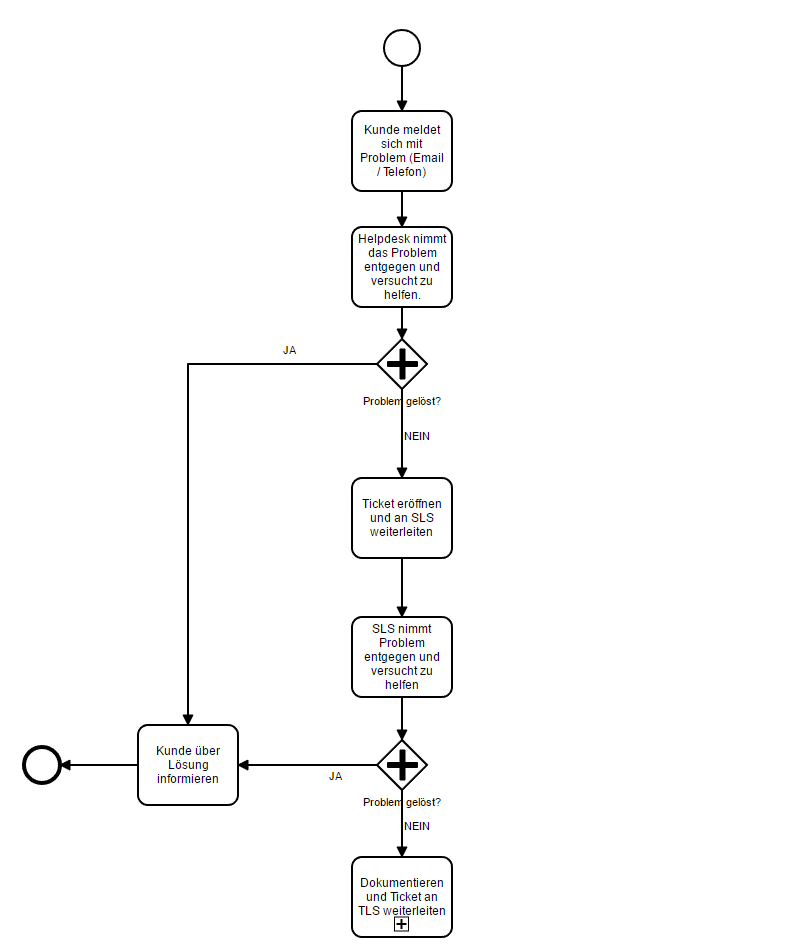
\includegraphics[width=0.80\textwidth]{images/support_process.PNG}
	\caption{Supportprozess des XYZ Softwarehauses}
	\label{fig:support-process}
\end{figure}

\subsection{Ablauf}
Der erste Schritt des Prozesses besteht aus der Anfrage eines Kunden oder einer Kundin. Dies geschieht meist per E-Mail, kann aber auch durch einen Telefonanruf erfolgen. Dabei entstehen abhängig vom gewählten Medium unterschiedliche Daten. Diese stellen sich entweder in Form von Lautsprache, oder als geschriebener Text dar. Im Folgenden wird ausschließlich auf die Anfrage per E-Mail eingegangen.

Der Helpdesk nimmt die Anfragen des Kunden entgegen und versucht das Problem zu lösen. Dazu stehen dem Helpdesk mehrere Möglichkeiten zur Verfügung. In den meisten Fällen wird der Mitarbeiter oder die Mitarbeiterin am Helpdesk versuchen, Informationen zu dem gemeldeten Problem in der Wissensbasis zu finden. Dazu wird die Wissensbasis durchsucht. Es werden Textausschnitte oder Schlagwörter verwendet die das Anliegen des Kunden möglichst gut wiedergeben. Wurde eine Lösung für das Problem gefunden, wird diese Lösung vom Helpdeskmitarbeiter oder der Helpdeskmitarbeiterin angewendet oder die Informationen direkt an den Kunden oder die Kundin weitergegeben. Falls keine Information in der Wissensbasis gefunden werden kann, wird versucht, das Problem durch implizites Wissen des Mitarbeiters oder der Mitarbeiterin zu lösen. Falls auf diesem Weg eine Lösung gefunden werden kann, wird der Mitarbeiter oder die Mitarbeiterin die Informationen zur Lösung in der Wissensbasis hinzufügen und den Kunden oder die Kundin über die Lösung des Problems informieren. Für jede Lösung wird dem Kunden oder der Kundin zusätzlich ein Link zu dem Artikel mit der Lösung in der Wissensbasis übermittelt. Dies führt im Idealfall dazu, dass der Kunde oder die Kundin in Zukunft ohne Hilfe des Helpdesks zu einer Lösung findet.

Kann auf Grund der Komplexität des Problems im ersten Schritt vom Helpdesk keine Lösung gefunden werden, wird überprüft, ob bereits ein Ticket für dieses Problem geöffnet wurde. Möglicherweise ist das gemeldete Problem bereits bei anderen Kunden aufgetreten und daher auch schon im Ticketsystem vermerkt. Dieses manuelle Auffinden der Tickets ist sehr häufig mit einem vermehrten Zeitaufwand verbunden und häufig werden doppelt erstellte Tickets erst spät entdeckt. Falls das Problem noch nicht in Form eines Tickets beschrieben wurde, wird ein Ticket erstellt, welches alle bereits vom Helpdesk erhaltenen Informationen enthält und an den sogenannten \textit{Second Level Support (SLS)} weitergeleitet wird. Wenn im SLS eine Lösung gefunden werden kann, folgen die gleichen Schritte wie bei erfolgreicher Abarbeitung im Helpdesk: Der Kunde oder die Kundin wird informiert und die Wissensbasis ergänzt. Zusätzlich wird dem Helpdesk eine Information gegeben, dass die Wissensbasis um die nötigen Informationen erweitert wurde, sodass bei zukünftigen Anfragen dieser Art eine Lösung möglicherweise schon von einem Mitarbeiter oder einer Mitarbeiterin des Helpdesks gefunden werden kann.

Wenn das Problem auch im SLS nicht gelöst werden kann, geht es schließlich zum sogenannten \textit{Third Level Support(TLS)}. Dieser Teil des Prozesses ist in Abbildung \ref{fig:support-process} nur als Subprozess modelliert, da er sich sehr ähnlich gestaltet wie der Prozessschritt im SLS. Das Ergebnis dieses Prozessschrittes ist erneut, die Rückmeldung an den Kunden oder die Kundin und die Erweiterung der Wissensbasis, sowie das Informieren des Helpdesks und des SLS über die Erweiterung.

Im Endeffekt sollte durch die kontinuierliche Erweiterung und Verbesserung der Wissensbasis ein System geschaffen werden, welches es ermöglicht, dass immer mehr Probleme direkt vom Kunden oder der Kundin selbst gelöst werden können. Es sollte auch dazu beitragen, dass mehr einfache Probleme direkt vom Helpdesk gelöst werden können, sodass der Kunde oder die Kundin schnellere Rückmeldungen bekommen und der SLS und der TLS entlastet werden. Vor allem technische Probleme werden sehr häufig nur im SLS oder im TLS lösbar sein, da im Helpdesk schlichtweg keine Zeit für die Lösung dieser bleibt. 

\subsection{Verbesserung 1 - Kategorisierung der Anfrage}
\label{sec:improvement1}
Die erste Verbesserung die im Zuge des Supportprozesses vorgenommen werden kann ist eine Kategorisierung der Anfrage. Die meisten E-Mail-Programme und Mailserver bieten bereits eine grundlegende Kategorisierung über sogenannte Regeln an. Diese Regeln entsprechen dabei sehr stark vereinfachten Boolschen Abfragen. Es kann zum Beispiel festgelegt werden, dass alle E-Mails die vom gleichen Absender oder der gleichen Absenderin kommen, in ein bestimmtes Unterverzeichnis verschoben werden. In Abbildung \ref{fig:outlook-rules} ist ein Dialog für das Festlegen von Regeln in \textit{Microsoft Office 2016} dargestellt. Diese regelbasierte Ansatz bietet bereits eine sehr einfache Möglichkeit für die Vorsortierung der Emails. Die Problematik die sich mit diesem Ansatz ergibt ist der Konfigurationsaufwand für das Erstellen dieser Regeln. Vor allem bei sehr vielen Regeln und großen Systemen wird dieser sehr groß und teilweise unüberschaubar. Auf Grund der Tatsache, dass mit diesen Regeln nur sehr einfache Regeln abgebildet werden können, ist es zum Beispiel nicht möglich, alle Emails von einer gemeinsamen Domain (microsoft.com) in ein Unterverzeichnis weiterzuleiten. Weiters gibt es keine Möglichkeiten die Mails auf den Inhalt zu prüfen und Regeln anzugeben, die dazu führen würden, dass Mails abhängig vom Inhalt kategorisiert und weitergeleitet werden.

\begin{figure}[ht]
	\centering
		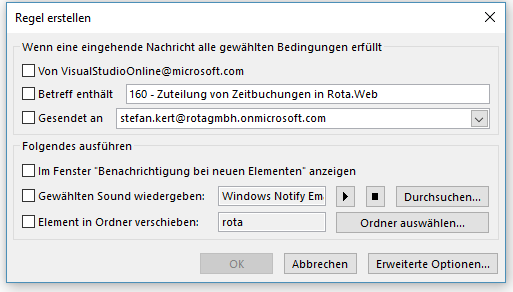
\includegraphics[width=0.80\textwidth]{images/outlook_rules.PNG}
	\caption{Dialog zum Festlegen von Regeln in MS Outlook}
	\label{fig:outlook-rules}
\end{figure}

Hier kann eine Anwendung von \textit{NLP} zum Beispiel dazu dienen, dass abhängig vom Inhalt der Email, eine Kategorie gefunden wird, in welche diese Email eingeordnet werden kann. Hier einige Beispiele für solche Kategorien:

\begin{itemize}
	\item Hardwareproblem
	\item Softwareproblem
	\item Verkauf Lizenzerweiterung
\end{itemize}
Die Email kann schließlich abhängig von der Kategorie zugeordnet werden und direkt an die gewünschten Stellen weitergeleitet werden. Das folgende Beispiel sollte zur Veranschaulichung dienen:

Kunde A stellt eine Anfrage über die Möglichkeiten der Lizenzerweiterung. Die Email geht direkt in den sogenannten \textit{Office-Posteingang} der als gemeinsames Postfach für das Unternehmen verwendet wird. Dieser Posteingang wird vom Helpdesk verwaltet. Nach dem Erhalt der Email wird ein Mitarbeiter oder eine Mitarbeiterin des Helpdesks diese Überprüfen und anschließend manuell in die Kategorie \textit{Verkauf Lizenzerweiterung} einordnen, wodurch die Email schließlich zum Vertrieb weitergeleitet wird.

Dieses Beispiel zeigt klar das Verbesserungspotential für diesen Prozess auf. Im Moment wird die Kategorisierung der Email manuell von einem Mitarbeiter oder einer Mitarbeiterin des Helpdesks vorgenommen. Diese Aufgabe könnte durch \textit{NLP} automatisiert erledigt werden, sodass der Aufwand für den Helpdesk hier sehr stark verringert wird.

\subsubsection{Vorteile}
Für diese Verbesserung ergeben sich folgende Vorteile:

\begin{itemize}
	\item Bessere Vorverarbeitung von Anfragen
	\item Automatisches Zuordnen und Kategorisieren von Anfragen
	\item Komplexere Regeln möglich
\end{itemize}

\subsubsection{Machbarkeit}
Die Kategorisierung von Daten ist eine Standardanwendung von \textit{NLP} und es gibt bereits zahlreiche Gebiete wo die Kategorisierung im Zusammenhang mit Text erfolgreich eingesetzt wird. Bei Kategorisierungen- oder Zuordnungsaufgaben werden im \textit{NLP} verschiedene sogenannte \textit{Clustering}- und \textit{Classification}-Methoden verwendet. 

Als Clustering wird die Möglichkeit bezeichnet,  Daten (meist auch als Dokumente bezeichnet) in Klassen oder Kategorien, sogenannte Cluster, von gleichen Daten zu gruppieren. Dabei sind beim Clustering zwei wichtige Kriterien zu erfüllen:

\begin{enumerate}
	\item Daten in einem Cluster sollten ähnlich sein
	\item Daten aus anderen Clustern sollten sich nicht ähneln.
\end{enumerate}
Das Zusammenfassen gleicher Daten zu neuen Gruppen ist das Ziel des \textit{Clusterings}. Die Aufgabe bei der \textit{Classification} besteht darin, dass im Gegensatz zum \textit{Clustering} eine Gruppierung der Daten auf Basis von vorgegebenen Kategorien statt. Die Gruppierung erfolgt also nicht auf Grund der vorhandenen Daten sondern die neuen Daten werden in vorgegebene Kategorien eingeordnet.

Ein Beispiel für die Anwendung von Clustering ist die Kategorisierung von wissenschaftlichen Artikeln, welche in dem Artikel \textit{Reconstructing the Giant: Automating the Categorization of Scientific Articles with Deep Learning Techniques} \cite{DannReconstructing} beschrieben wird. Die \textit{Clustering}-Methode, die im Artikel beschrieben wird, ist das \textit{Hirarchical Agglomerative Clustering (HAC)}. Dieses Verfahren zeichnet sich dadurch aus, dass es am Anfang alle Dokumente der Datenbasis in eigene \textit{Cluster} einordnet. Es wird für jeden dieser Cluster der ähnlichste Cluster gewählt und diese beiden Cluster formen einen neuen Cluster. Diese Verfahren wird rekursiv durchgeführt und verarbeitet alle Cluster, bis alle Artikel zu einem gemeinsamen Cluster zusammengefasst wurden. In dem genannten Artikel wird das Modell außerdem durch einen \textit{Deep-Learning} Technik trainiert. 

Eine Anwendung von \textit{Clustering} wäre für die Verbesserung in diesem Prozess grundsätzlich möglich, da bereits vordefinierten Kategorien von Anfragen existieren, ist die Anwendung von \textit{Classification}-Methoden hier zu empfehlen. 

In dem Buch \textit{Encyclopedia of Language \& Linguistics} wird eine Möglichkeit für die Anwendung von Classification-Methoden im Zusammenghang mit Texten beschrieben \cite{brown2006encyclopedia}. Bei der \textit{Classification} wird grundsätzlich zwischen der \textit{Single-Label-Classification} und der \textit{Multi-Label-Classification} unterschieden. Der Unterschied zwischen diese beiden Verfahren besteht darin, dass bei der \textit{Single-Label-Classification} nur eine Klasse zugeordnet wird, wohingegen bei der \textit{Multi-Label-Classification} mehrere Klassen zugeordnet werden können. In dem aktuellen Anwendungsfall, der dazu dienen sollte die Zuordnung von Anfragen zu bestimmten Kategorien zu finden, ist in erster Linie die \textit{Single-Label-Classification} von Interesse, da für diesen Prozess davon ausgegangen wird, dass die Anfragen immer nur an eine Stelle weitergeleitet und somit nur einer Kategorie zugeordnet werden. Für die Auswahl der  \textit{classification} Methode empfiehlt das Buch \textit{Encyclopedia of Language \& Linguistics} die Anwendung von Vektormaschinen beziehungsweise Boosting \cite{brown2006encyclopedia}. Die Hauptgründe für die Auswahl dieser beiden Verfahren sind die Genauigkeit, sowie die sehr gute Performance im Zusammenhang mit der Klassifizierung von Text. 

Auch hier ist es wieder erforderlich, dass das initiale Modell trainiert wird, sodass eine zukünftige Klassifizierung der Anfragen mit einer hohen Genauigkeit erfolgen kann. Die Datenbasis für das initiale Trainieren des Modells besteht dabei aus den bereits manuell zugeordneten Anfragen. Dabei ist es von enormer Wichtigkeit, dass für die Trainingsdaten richtig zugeordnete Anfragen verwendet werden, um das Primärziel, eine genaue Zuordnung zukünftiger Anfragen, zu erfüllen. Es sollte schlussendlich möglich sein, weitere Zuordnung basierend auf dem trainierten Modell zu finden und automatisiert zu verarbeiten.

\subsection{Verbesserung 2 - Hinzufügen von Informationen aus der Wissensbasis und Verknüpfen mit Anfragen aus der Vergangenheit}
\label{sec:improvement2}
Ein zentraler Bestandteil des Prozesses, ist die kontinuierliche Erweiterung der Wissensbasis, sowie die Verwendung der darin enthaltenen Informationen. Im Moment wird versucht, durch manuelles Durchsuchen dieser Wissensbasis, Informationen, die zum Lösen eines Problems beitragen, zu erhalten. Dies ist meist mit einem erhöhten Aufwand verbunden. Die Mitarbeiterin oder der Mitarbeiter des Helpdesks muss die Wissensbasis nach den Schlagwörtern, oder Inhalten die in der Anfrage enthalten sind durchsuchen, die Informationen ihrer Relevanz nach beurteilen und schließlich, die Ergebnisse in eine Antwort für die Kundin oder den Kunden umformen. Diese Vorgehensweise liefert sehr häufig gute Ergebnisse die genau auf das Problem des Kunden zugeschnitten sind, benötigt aber mehr Zeit für die Abarbeitung. 

Ein weiterer Teil dieser Verbesserung besteht in der Zuordnung von Fällen aus der Vergangenheit die ähnlich sind wie die aktuelle Anfrage. Ähnlich wie beim Auffinden der Informationen in der Wissensbasis kann hier durch die Anwendung von \textit{NLP} ein Vergleich zu den Anfragen aus der Vergangenheit gezogen werden und diese für den Mitarbeiter oder die Mitarbeiterin des Helpdesks zur Verfügung gestellt werden. Der Vorteil besteht darin, dass selbst wenn keine Informationen in der Wissensbasis vorhanden sind, trotzdem Informationen aus bereits gelösten Fällen bezogen werden können.

Mit Hilfe von \textit{NLP} kann eine teilweise Automatisierung des Durchsuchen der Wissensbasis, beziehungsweise Zuordnung zu Anfragen aus der Vergangenheit erreicht werden. Die Anfragen, welche für den Support bestimmt sind und Probleme darstellen, werden mit Informationen aus der Wissensbasis und älteren Anfragen verglichen. Dieser Vergleich kann mehrere unterschiedliche Ergebnisse liefern. Vereinfacht gesagt, werden die Anfragen und die Informationen aus der Wissensbasis und den älteren Anfragen in Kategorien aufgeteilt. Dies ist grundsätzlich sehr ähnlich zu der Verbesserung in Abschnitt \ref{sec:improvement1}, ein sehr zentraler Unterschied besteht aber darin, dass die Anfragen mehreren Kategorien zugeordnet werden müssen und das die Kategorien initial noch nicht vorhanden sind. Die Kategorien müssen erst aus den vorhandenen Informationen aus der Wissensbasis und aus Anfragen aus der Vergangenheit gebildet werden. 

Die Zuordnung zu mehreren Kategorien hat in erster Linie den Hintergrund, dass Probleme sich häufig nicht eindeutig in eine Kategorie passen. Meist erstreckt sich ein Problem über mehrere Kategorien. In diesem Fall, würde eine sogenannten \textit{harte Zuordnung}, wodurch eine Zuordnung nur zu einer Kategorie möglich ist nicht ausreicht. Weiters kommt es sehr häufig vor, dass Kunden mehrere Probleme in einer Anfrage beschreiben, oder die Probleme einen Zusammenhang mit anderen Kategorien haben, dir für das ermitteln der Lösung von Bedeutung ist.

Wenn die Zuordnung zu einer oder mehreren Kategorien erfolgt ist, können die Informationen aus der Wissensbasis, sowie die Informationen aus den älteren Anfragen, welche der gleichen Kategorie wie die Anfrage zugeordnet sind, ermittelt werden. Hier wäre eine weitere Möglichkeit zur Reihung dieser Ergebnisse, dass eine Sortierung nach der Relevanz der einzelnen gefunden Informationen erfolgt. Das Ergebnis ist eine der Relevanz nach sortierte Liste an Informationen.

Der Mitarbeiter oder die Mitarbeiterin des Helpdesks hat nun die Möglichkeit, dem Kunden oder der Kundin eine Information aus dem erhaltenen Ergebnis zurückzusenden, wodurch noch eine weitere manuelle Überprüfung der erhaltenen Informationen auf Korrektheit möglich ist. 

Hier wäre es möglich, durch die Rückgabe der Auswahl der Information durch den Mitarbeiter oder die Mitarbeiterin des Helpdesks, das Modell für die Kategorisierung weiter zu trainieren. Wenn beispielsweise keiner der Artikel zu der gestellten Anfrage passt, kann durch zwei Schritte Einfluss auf das Modell genommen werden. Im ersten Schritt sollte die Kategorie überprüft werden, welcher die Anfrage zugeordnet wurde. Falls diese Zuordnung falsch ist, muss eine manuelle Zuordnung zu einer passenden Kategorie erfolgen. Diese Zuordnung sollte in jedem Fall wieder ins Modell zurückfließen, sodass die Anfragen in Zukunft besser zugeordnet werden. Der zweite Schritt ist eine manuelle Suche durch den Mitarbeiter oder die Mitarbeiterin des Helpdesks. Das Ergebnis dieser manuellen Suche kann ebenfalls zum trainieren des Modells verwendet werden. Im Idealfall führt dies zu besseren Suchergebnissen in der Zukunft.

Dieses Trainieren des Models kann schließlich auch bei der manuelle Suche in der Wissensbasis unterstützen, von dem schlussendlich auch Kunden und die Mitarbeiter und Mitarbeiterinnen des Helpdesks profitieren, da die Ergebnisse, die zu Anfragen gefunden werden, durch das Trainieren des Modells immer genauer werden.

Als weiterer Optimierungsschritt für den Prozessablauf wird dem Mitarbeiter oder der Mitarbeiterin des Helpdesks die Möglichkeit gegeben, aus der erhaltenen Informationen, welche als Ergebnis der automatischen Suche geliefert wurde, eine E-Mail generieren zu lassen, die alle Informationen, wie Links, Beschreibungen oder weiterführende Informationen enthält.

Ein weiterer Schritt, der zu einer Verbesserung des Modells und der Wissensbasis beitragen kann, ist das miteinbeziehen der Rückmeldung des Kunden oder der Kundin. Dem Kunden oder der Kundin wird über eine Bewertungs- und eine Kommentarfunktion die Möglichkeit gegeben, die erhaltenen Informationen zu bewerten. Diese Information kann nach einer Prüfung durch einen Mitarbeiter oder eine Mitarbeiterin des Helpdesks wieder ins Modell integriert werden und so das Modell weiter trainieren. Hier, wie auch bei der Auswahl durch den Mitarbeiter oder die Mitarbeiterin des Helpdesks, besteht natürlich die Gefahr, dass das Modell mit falschen Informationen trainiert wird und dadurch die Ergebnisse in Zukunft verschlechtert werden. Um diese Problematik so gering wie möglich zu halten, erfordert es eine hohe Genauigkeit beim weitergeben der Informationen an das Modell.


\subsubsection{Vorteile}
Für diese Verbesserung ergeben sich folgende Vorteile:

\begin{itemize}
	\item Schnelles und automatisches Erhalten von Informationen aus der Wissensbasis
	\item Geringer manueller Aufwand für Helpdesk
	\item Manuelle Suche wird durch Trainieren des Models verbessert
	\item Auffinden bereits behandelter Anfragen
\end{itemize}

\subsubsection{Machbarkeit}
Wie bereits in Abschnitt \ref{sec:improvement1} kann auch hier auf bereits vorhandenen Algorithmen und Vorgehensweisen für die Kategorisierung von Texten zurückgegriffen werden. Auf Grund der Tatsache, dass es sehr viele Kategorien von Problemen gibt und Anfragen auch mehrere Probleme beinhalten können, sowie die Tatsache, dass sich Probleme auf mehrere Kategorien verteilen können, ist die Komplexität dieser Verbesserung signifikant höher als die Verbesserung in Abschnitt \ref{sec:improvement1}.

Grundsätzlich wäre hier das Verwenden einer \textit{Classification}-Methode möglich. Um die Anforderung der Zuordnung zu mehreren Kategorien zu erfüllen, kann hier auf eine sogenannte \textit{Multi-Label-Classification} gesetzt werden. Da für diese Verbesserung keine Datenbasis vorhanden ist, die eine Zuordnung zu vorgegebenen Kategorien ermöglicht, ist für diese Verbesserung die Anwendung einer \textit{Clustering}-Methode empfehlenswert.

Für den Fall, dass eine Zuordnung mittels Clustering erfolgen sollte, ist die Anwendung von \textit{Fuzzy-Clustering}-Methoden notwendig. \textit{Fuzzy-Clustering}-Methoden ermöglichen die Zuordnung von Daten zu mehreren verschiedenen Clustern. Ein Beispiel für die Anwendung von \textit{Fuzzy-Clustering}-Methoden im Zusammenhang mit Text ist in dem Artikel \textit{A Scalable Hierarchical Fuzzy Clustering Algorithm for Text Mining} beschrieben \cite{rodrigues2004scalable}. Das in diesem Artikel beschrieben Problem ist dem Problem, welches mit dieser Verbesserung gelöst werden sollte sehr ähnlich. Die Anwendung, die beschrieben wird, behandelt die Zuordnung von Themen zu unterschiedlichen Domänen. Dabei hängen Themen, die sich auf eine bestimmte Domäne beziehen, mit anderen Themen aus dieser Domäne zusammen und stehen in einer Beziehung zu diesen. Häufig beziehen sich Themen auch auf andere Domänen und sind daher auch für diese anderen Domänen mehr oder weniger relevant. Gleich wie bei dem Problem, welches sich im Zusammenhang mit den Problemkategorien ergibt, müssen also Themen mehren Domänen gleichzeitig zugeordnet werden. Durch die Anwendung von \textit{Fuzzy-Clustering} Methoden kann eben dieses Problem gelöst werden. Die Themen können gleichzeitig mehreren Domänen zugeordnet werden, wodurch sich teilweise hilfreiche Beziehungen zwischen den einzelnen Domänen und Themen ergeben, die bei einem normalen \textit{clustering} nicht ersichtlich wären.

Durch das \textit{Clustering} können neue Anfragen in Cluster eingeordnet werden. Diese Cluster beinhalten dabei Artikel aus der Wissensbasis, sowie Anfragen aus der Vergangenheit. Durch diese Zuordnung können die erwähnten Vorteile erzielt werden, und es ist dem Mitarbeiter oder der Mitarbeiterin des Helpdesks möglich, abhängig von der Anfrage, sich auf Informationen aus der Wissensbasis, sowie auf Informationen aus Anfragen aus der Vergangenheit zu beziehen.

Eine Herausforderung die sich im Zusammenhang mit dieser Verbesserung ergibt, ist das befüllen der Wissensbasis. Wenn diese nur unzureichend befüllt ist, oder überhaupt nicht vorhanden, werden sich die durch diese Verbesserung beschriebenen Vorteile für das Unternehmen nur sehr begrenzt ergeben. Für diesen Fall bietet diese Verbesserung immer noch die Möglichkeit, Lösungen für neue Anfragen, in Anfragen aus der Vergangenheit zu erhalten, da diese dem Cluster der aktuellen Anfrage zugeordnet sind.

Um den erwähnten Vorteil der Relevanz zu erzielen, muss für die \textit{Clustering} Methode zusätzlich eine Möglichkeit gefunden werden, die Relevanz der Information mit einfließen zu lassen. Dies kann eben über den erwähnten manuellen Input durch Mitarbeiter oder Mitarbeiterinnen des Helpdesks oder auch den Kunden erfolgen. Das Modell für die Suche der Daten sollte im Idealfall laufend trainiert werden, sodass die Ergebnisse im Laufe der Zeit immer besser werden. Dies bedeutet vor allem am Anfang einen erhöhten manuellen Aufwand. Häufig gibt es bereits eine Auswertung wie hilfreich gewisse Informationen aus der Wissensbasis sind, dies kann natürlich für das Reihen der Informationen nach Relevanz verwendet werden.

\subsection{Verbesserung 3 - Erkennen von duplizierten Tickets}
Kann das Problem von einem Mitarbeiter oder einer Mitarbeiterin des Helpdesk nicht gelöst werden, wird ein sogenanntes Ticket erstellt. Dieses Ticket enthält Informationen über das Problem, den Kunden oder die Kundin, wo das Problem aufgetreten ist und weitere Metainformationen wie Betriebssystem, Version der Applikation, oder auch ob das Problem nur zu einer bestimmten Uhrzeit auftritt. Vor der Erstellung dieses Tickets, wird das Ticketsystem noch auf ähnliche Probleme durchsucht. In manchen Fällen lassen sich bei dieser Suche bereits ähnliche Fälle für dieses Problem finden. Ist dies der Fall wird das neue Ticket mit dem alten Ticket verknüpft, sodass beide gemeinsam gelöst werden können. Dieser Schritt erfordert erneut eine manuelle Suche die durch einen Mitarbeiter oder eine Mitarbeiterin des Helpdesks erfolgen muss. Hier könnte eine Verbesserung durch die Anwendung von \textit{NLP} dadurch erreicht werden, dass sobald ein Ticket erstellt wird, die Wissensbasis automatisch nach ähnlichen oder gleichen Tickets durchsucht wird. Es sollten also Duplikate von Tickets erkannt werden und dem Mitarbeiter oder der Mitarbeiterin eine Rückmeldung gegeben werden, dass dieses oder ein ähnliches Ticket bereits erstellt wurde und ob diese Tickets verknüpft werden sollten. Auch hier ist eine manuelle Eingabe des Mitarbeiters oder der Mitarbeiterin erforderlich. Der Mitarbeiter oder die Mitarbeiterin prüft, ob die ermittelten Ergebnisse wirklich übereinstimmen. Ist dies der Fall, wird das Ticket zugeordnet.

Eine weitere Möglichkeit im Zuge dieser Verbesserung, ist das in Abschnitt \ref{sec:improvement2} beschrieben Verfahren zum Auffinden von ähnlichen Anfragen. Die Tickets, welche diesen ähnlichen Anfragen zugeordnet sind können als potentielle Duplikate des aktuellen Tickets in Betracht gezogen werden. Die Zuordnung erfolgt abhängig davon, ob das Ticket bereits abgeschlossen ist oder nicht. Falls das Ticket bereits abgeschlossen wurde, wird dem Mitarbeiter oder der Mitarbeiterin die Information gegeben, dass bereits eine Lösung vorhanden ist. Falls nicht kann erneut eine Verknüpfung der Tickets durch ein manuelles Eingreifen des Mitarbeiters oder der Mitarbeiterin erfolgen.

\subsubsection{Vorteile}
Für diese Verbesserung ergeben sich folgende Vorteile:

\begin{itemize}
	\item Schnelles und automatisches Auffinden von duplizierten Tickets
	\item Weniger Tickets weden zum SLS oder zum TLS weitergeleitet, da duplizierte Tickets bereits zuvor zusammengefasst werden
\end{itemize}

\subsubsection{Machbarkeit}
Für das Auffinden von Duplikaten ergeben sich die gleichen Anforderungen wie für die Verbesserung in Abschnitt \ref{sec:improvement2}. Auch hier müssen ähnliche Dokumente (Tickets) gruppiert werden, sodass diese verlinkt werden können. Dabei empfiehlt sich erneut die Verwendung einer \textit{Clustering}-Methode. Genau wie bei der Verbesserung in Abschnitt \ref{sec:improvement2}, beschränken sich die Tickets meist nicht auf einen Cluster, sondern können mehreren Clustern zugeordnet sein. Eine weitere Möglichkeit für den Vergleich ist die Anwendung der sogenannten \textit{Cosinus-Similarity} \cite{steinbach2000comparison}. Dabei gibt die \textit{Cosinus-Similarity} an, wie ähnlich sich zwei Tickets sind. Dies wird ermittelt, indem der Winkel zwischen zwei Vektoren, welche die einzelnen Tickets repräsentieren, berechnet wird. Der erhaltene Wert gibt Aufschluss über die Ähnlichkeit. 

Beim Training kann für diese Anwendung auf die gesamte Datenbasis der vorhandenen Tickets zurückgegriffen werden. Mit Hilfe einer \textit{Clustering}-Methode werden sämtliche Tickets in Cluster eingeordnet, sodass das initiale Modell entsteht. Neue Tickets werden diesen Clustern zugeordnet und werden somit gemeinsam mit ähnlichen Tickets gruppiert. In einer einfachen Ausbaustufe dieser Verbesserung könnten auf eine Anfrage nach ähnlichen Tickets, alle Tickets eines Clusters gelistet werden. Der Mitarbeiter oder die Mitarbeiterin des Helpdesks hat daraufhin die Möglichkeit, eine manuelle Auswahl der Duplikate vorzunehmen. In einer späteren Ausbaustufe, kann zusätzlich zwischen den einzelnen Tickets verglichen werden und kleinere Cluster gebildet werden, sodass nur noch bei einer sehr starken Ähnlichkeit eine Zuordnung erfolgen kann.
